%-------------------------------------------------------%
\section{Overview} \label{sec:tutrial_real_intro}
%-------------------------------------------------------%
In this chapter, the basic execution procedure of the real atmospheric experiment is described using a simple case according to the workflow in Fig. \ref{fig:howto}.
\begin{enumerate}
\item Preparations for input data. The input data must be prepared by users themselves.
\item \texttt{pp}:   Making topographical data
\item \texttt{init}: Making initial and boundary data
\item \texttt{run}:  Executing the simulation
\item \texttt{net2g}: Converting {\netcdf} output data to {\grads} format ( optional )
\end{enumerate}
Hereinafter, the absolute path \texttt{scale-{\version}/scale-rm/test/tutorial/} is denoted by\\
\verb|${Tutorial_DIR}|.

\begin{figure}[tb]
\begin{center}
  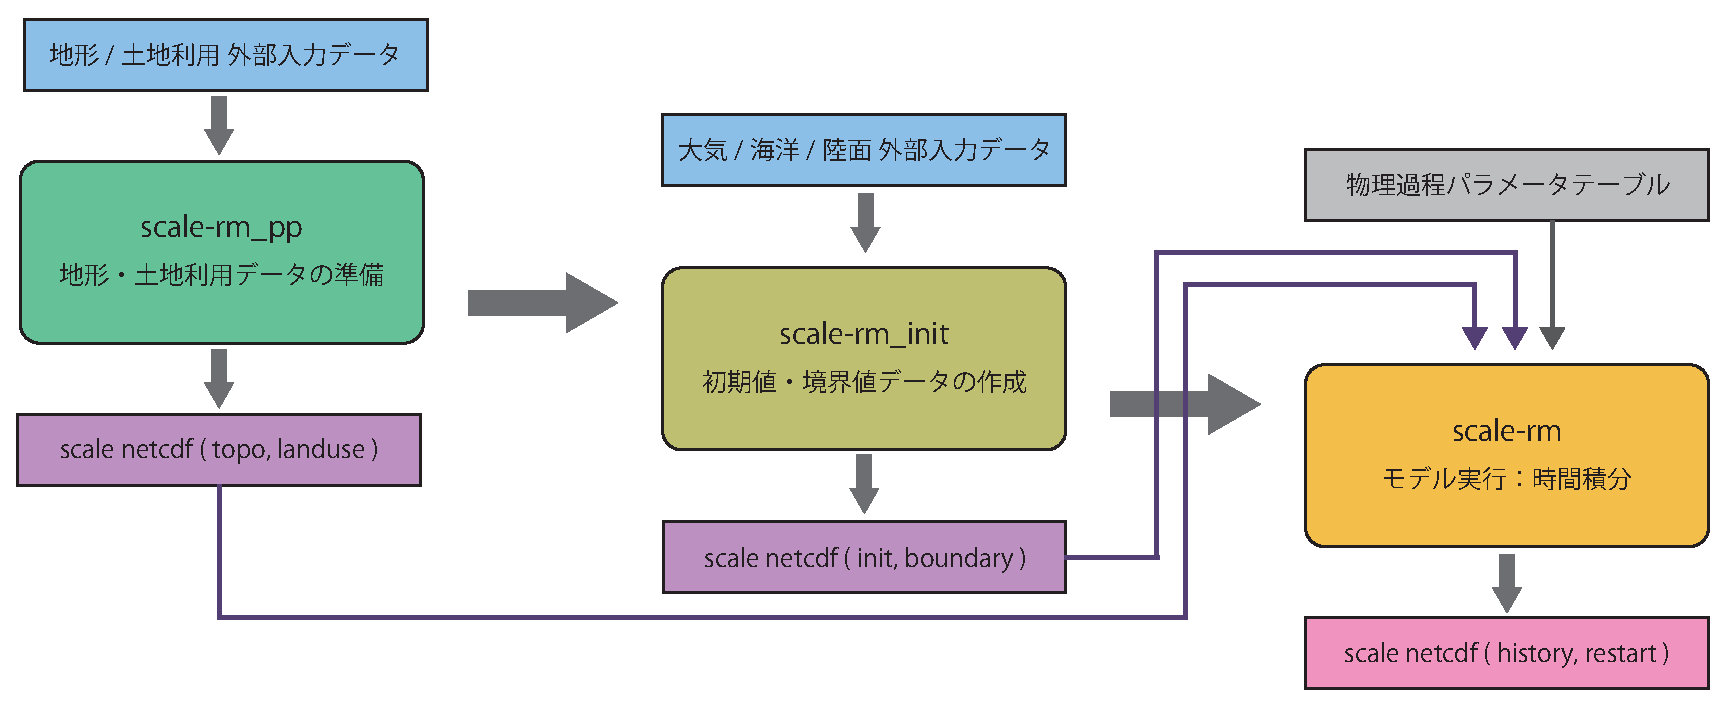
\includegraphics[width=0.9\hsize]{./figure/real_procedure.eps}\\
  \caption{\scalerm procedure of model execution}
  \label{fig:howto}
\end{center}
\end{figure}

The settings for the calculation domain used in this tutorial are given in Table \ref{tab:grids}.
Figure \ref{fig:tutrial_real_domain} shows the target domain.
Since this tutorial focuses on learning how to conduct 
real atmospheric experiments using \scalerm quickly,
the experiment is designed to be completed in a short time.
Note that this setting may not be appropriate as a physically valid experiment;
e.g., there is no cumulus parameterization in this simulation, even though the horizontal resolution is 20 km.

\begin{table}[tb]
\begin{center}
  \caption{Overview of experimental settings}
  \label{tab:grids}
  \begin{tabularx}{150mm}{|l|X|} \hline
    \rowcolor[gray]{0.9} Item & Configuration \\ \hline
    MPI process decomposition (east-west $\times$ north-south) & 2 $\times$ 2 (total: 4 processes) \\ \hline
    Number of horizontal grids (east-west $\times$ north-south) & 90 $\times$ 90  \\ \hline
    Number of vertical layers   & 36                   \\ \hline
    Horizontal grid intervals   & $\Delta x  = \Delta y = $ 20km       \\ \hline
    Integration period & July 14, 2007, 18UTC - July 15 00UTC (6 hour integration) \\ \hline
    Time step & 90 s/step (total:240 steps) \\ \hline
  \end{tabularx}
\end{center}
\end{table}

\begin{figure}[tb]
\begin{center}
  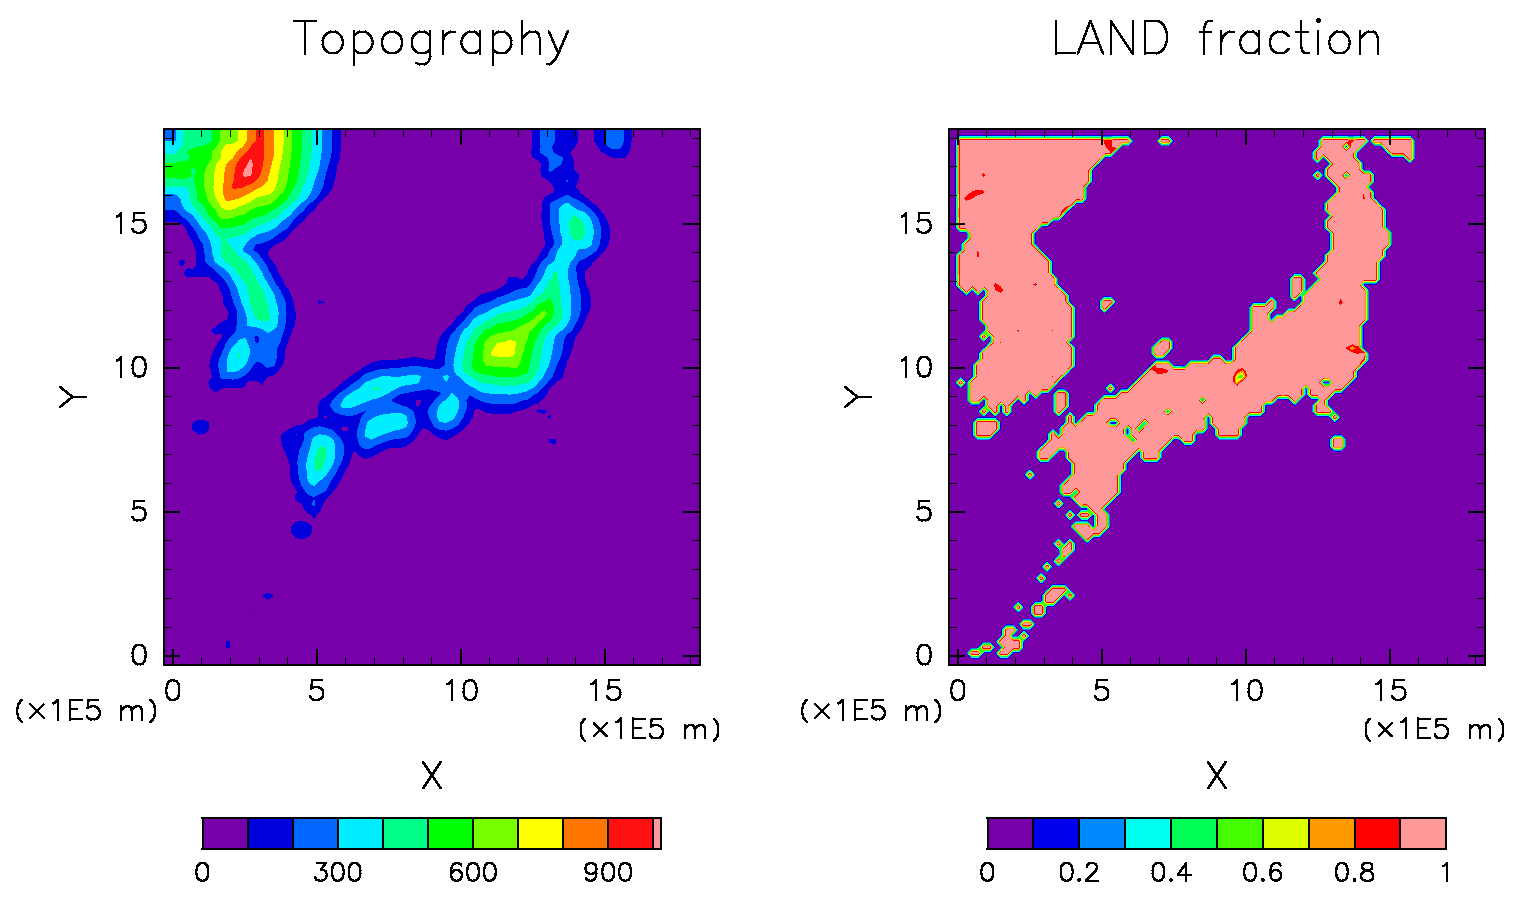
\includegraphics[width=1.0\hsize]{./figure/real_domain.eps}\\
  \caption{Topographical and land-ocean distribution in the domain}
  \label{fig:tutrial_real_domain}
\end{center}
\end{figure}


